\documentclass[a4paper]{article}
\usepackage{times}
\usepackage[utf8]{inputenc}
\usepackage{selinput}
\usepackage{upquote}
\usepackage[margin=2cm, rmargin=4cm, tmargin=3cm]{geometry}
\usepackage{tcolorbox}
\usepackage{xspace}
\usepackage[french]{babel}
\usepackage{url}
\usepackage{hyperref}
\usepackage{fontawesome5}
\usepackage{marginnote}
\usepackage{ulem}
\usepackage{tcolorbox}
\usepackage{graphicx}
%\usepackage[top=Bcm, bottom=Hcm, outer=Ccm, inner=Acm, heightrounded, marginparwidth=Ecm, marginparsep=Dcm]{geometry}


\newtcolorbox{Example}[1]{colback=white,left=20pt,colframe=slideblue,fonttitle=\bfseries,title=#1}
\newtcolorbox{Solutions}[1]{colback=white,left=20pt,colframe=green,fonttitle=\bfseries,title=#1}
\newtcolorbox{Conseils}[1]{colback=white,left=20pt,colframe=slideblue,fonttitle=\bfseries,title=#1}
\newtcolorbox{Warning}[1]{colback=white,left=20pt,colframe=warning,fonttitle=\bfseries,title=#1}

\setlength\parindent{0pt}

  %Exercice environment
  \newcounter{exercice}
  \newenvironment{Exercice}[1][]
  {
  \par
  \stepcounter{exercice}\textbf{Question \arabic{exercice}:} (\faClock \enskip \textit{#1})
  }
  {\bigskip}
  

% Title
\newcommand{\titre}{\begin{center}
  \section*{Algorithmes et Pensée Computationnelle}
\end{center}}
\newcommand{\cours}[1]
{\begin{center} 
  \textit{#1}\\
\end{center}
  }


\newcommand{\exemple}[1]{\newline~\textbf{Exemple :} #1}
%\newcommand{\attention}[1]{\newline\faExclamationTriangle~\textbf{Attention :} #1}

% Documentation url (escape \# in the TP document)
\newcommand{\documentation}[1]{\faBookOpen~Documentation : \href{#1}{#1}}

% Clef API
\newcommand{\apikey}[1]{\faKey~Clé API : \lstinline{#1}}
\newcommand{\apiendpoint}[1]{\faGlobe~Url de base de l'API \href{#1}{#1}}

%Listing Python style
\usepackage{color}
\definecolor{slideblue}{RGB}{33,131,189}
\definecolor{green}{RGB}{0,190,100}
\definecolor{blue}{RGB}{121,142,213}
\definecolor{grey}{RGB}{120,120,120}
\definecolor{warning}{RGB}{235,186,1}

\usepackage{listings}
\lstdefinelanguage{texte}{
    keywordstyle=\color{black},
    numbers=none,
    frame=none,
    literate=
           {é}{{\'e}}1
           {è}{{\`e}}1
           {ê}{{\^e}}1
           {à}{{\`a}}1
           {â}{{\^a}}1
           {ù}{{\`u}}1
           {ü}{{\"u}}1
           {î}{{\^i}}1
           {ï}{{\"i}}1
           {ë}{{\"e}}1
           {Ç}{{\,C}}1
           {ç}{{\,c}}1,
    columns=fullflexible,keepspaces,
	breaklines=true,
	breakatwhitespace=true,
}
\lstset{
    language=Python,
	basicstyle=\bfseries\footnotesize,
	breaklines=true,
	breakatwhitespace=true,
	commentstyle=\color{grey},
	stringstyle=\color{slideblue},
  keywordstyle=\color{slideblue},
	morekeywords={with, as, True, False, Float, join, None, main, argparse, self, sort, __eq__, __add__, __ne__, __radd__, __del__, __ge__, __gt__, split, os, endswith, is_file, scandir, @classmethod},
	deletekeywords={id},
	showspaces=false,
	showstringspaces=false,
	columns=fullflexible,keepspaces,
	literate=
           {é}{{\'e}}1
           {è}{{\`e}}1
           {ê}{{\^e}}1
           {à}{{\`a}}1
           {â}{{\^a}}1
           {ù}{{\`u}}1
           {ü}{{\"u}}1
           {î}{{\^i}}1
           {ï}{{\"i}}1
           {ë}{{\"e}}1
           {Ç}{{\,C}}1
           {ç}{{\,c}}1,
    numbers=left,
}

\newtcbox{\mybox}{nobeforeafter,colframe=white,colback=slideblue,boxrule=0.5pt,arc=1.5pt, boxsep=0pt,left=2pt,right=2pt,top=2pt,bottom=2pt,tcbox raise base}
\newcommand{\projet}{\mybox{\textcolor{white}{\small projet}}\xspace}
\newcommand{\optionnel}{\mybox{\textcolor{white}{\small Optionnel}}\xspace}
\newcommand{\advanced}{\mybox{\textcolor{white}{\small Pour aller plus loin}}\xspace}
\newcommand{\auto}{\mybox{\textcolor{white}{\small Auto-évaluation}}\xspace}


\usepackage{environ}
\newif\ifShowSolution
\NewEnviron{solution}{
  \ifShowSolution
	\begin{Solutions}{\faTerminal \enskip Solution}
		\BODY
	\end{Solutions}
  \fi}


  \usepackage{environ}
  \newif\ifShowConseil
  \NewEnviron{conseil}{
    \ifShowConseil
    \begin{Conseils}{\faLightbulb \quad Conseil}
      \BODY
    \end{Conseils}

    \fi}

    \usepackage{environ}
  \newif\ifShowWarning
  \NewEnviron{attention}{
    \ifShowWarning
    \begin{Warning}{\faExclamationTriangle \quad Attention}
      \BODY
    \end{Warning}

    \fi}
  

%\newcommand{\Conseil}[1]{\ifShowIndice\ \newline\faLightbulb[regular]~#1\fi}



\usepackage{listings}
\usepackage{array}
\newcolumntype{C}[1]{>{\centering\let\newline\\\arraybackslash\hspace{0pt}}m{#1}}

\begin{document}

% Change the following values to true to show the solutions or/and the hints
\ShowSolutiontrue
\ShowConseiltrue
\titre
\cours{Algorithmes de tri et Complexité - exercices avancés}

Le but de cette série d'exercices est d'aborder les notions présentées durant la séance de cours. Cette série d'exercices sera orientée autour des points suivants:

\begin{enumerate}
    \item la complexité des algorithmes,
    \item la récursivité et
    \item les algorithmes de tri
\end{enumerate}

Les languages de programmation qui seront utilisés pour cette série d'exercices sont Java et Python.

Le temps indiqué (\faClock) est à titre indicatif.

\section{Récursivité (5 minutes) }
\begin{Exercice}[5 minutes] \textbf{Somme des chiffres} \\
    Écrivez un algorithme récursif en Python ou en Java qui prend un nombre et retourne la somme des chiffres dont il est composé. Par exemple, la somme des chiffres de 126 est : 1+2+6 = 9.
    
    \begin{conseil}
    
    Pour obtenir les chiffres qui composent un nombre, utilisez l'opérateur \lstinline{\%} (modulo - \url{https://fr.wikipedia.org/wiki/Modulo\_(op\%C3\%A9ration)}). \\
    Pour obtenir le nombre 12 à partir du nombre 126, il vous suffit de faire la division entière par 10. En Python, on utilise l'opérateur \lstinline{\/\/} : 126 \lstinline{\/\/} 10 = 12. En Java, la division entre deux variables de type \lstinline{int} est entière, et vous n'aurez ainsi qu'à utiliser l'opérateur de division normal \lstinline{\/} : 126 \lstinline{\/} 10 = 12.
    
    \end{conseil}
    
    \begin{solution}
    \textbf{Python :}
        \lstinputlisting{solutions/question6.py}
                
    \textbf{Java :}
       \lstinputlisting{solutions/question6.java}
    
    \end{solution}
\end{Exercice}

\section{Algorithmes de Tri (60 minutes)}

\begin{Exercice} [20 minutes] \textbf{Tri à bulles (Bubble Sort) - java} \\
Le tri à bulles consiste à parcourir une liste et à comparer ses éléments. Le tri est effectué en permutant les éléments de telle sorte que les éléments les plus grands soient placés à la fin de la liste. 

Concrètement, si un premier nombre $x$ est plus grand qu'un deuxième nombre $y$ et que l'on souhaite trier l'ensemble par ordre croissant, alors $x$ et $y$ sont mal placés et il faut les inverser. Si, au contraire, $x$ est plus petit que $y$, alors on ne fait rien et l'on compare $y$ à $z$, l'élément suivant.

Soit la liste \lstinline{l = [1, 2, 4, 3, 1]}, triez les éléments de la liste en utilisant un tri à bulles. Combien d'itérations effectuez-vous?

\begin{itemize}
        \item \textbf{Java :}
            \lstinputlisting{ressources/question8.java} 
    \end{itemize}
    
    \begin{conseil}
    En Java, utilisez une variable temporaire que vous nommerez \lstinline{temp} afin de faire l'échange de valeur entre deux éléments de la liste.
    \end{conseil}
    
    \ \\
    
    \begin{solution}
    \textbf{Java:}
    \lstinputlisting{solutions/question8.java} 


    L'algorithme a une complexité de $O(n^2)$ car il contient deux boucles qui parcourent la liste.\\\\\\
            
\end{solution}
\end{Exercice}

\begin{Exercice} [20 minutes] \textbf{Tri par insertion - 2 (Insertion Sort)} \\

    Dans l'algorithme de tri par insertion, on parcourt le tableau à trier du début à la fin. Au moment où on considère le i-ème élément, les éléments qui le précèdent sont déjà triés. Pour faire l'analogie avec l'exemple du jeu de cartes, lorsqu'on est à la i-ème étape du parcours, le i-ème élément est la carte saisie, les éléments précédents sont la main triée et les éléments suivants correspondent aux cartes encore en désordre sur la table. 
    
    L'objectif d'une étape est d'insérer le i-ème élément à sa place parmi ceux qui le précède. Il faut pour cela trouver où l'élément doit être inséré en le comparant aux autres, puis décaler les éléments afin de pouvoir effectuer l'insertion. En pratique, ces deux actions sont fréquemment effectuées en une passe, qui consiste à faire ``remonter'' l'élément au fur et à mesure jusqu'à rencontrer un élément plus petit. 
    
    Compléter le code suivant pour trier la liste \lstinline{l} définie ci-dessous en utilisant un tri par insertion. Combien d'itérations effectuez-vous?
    \begin{itemize}
        \item \textbf{Python :}
            \lstinputlisting{ressources/question10.py} 
        \item \textbf{Java :}
            \lstinputlisting{ressources/question10.java} 
    \end{itemize}
    
    \begin{conseil}
        Référez vous à la figure du dessous pour un exemple de tri par insertion. \\
        Référez vous aussi aux diapositives 18 à 72 du cours.
    \end{conseil}
    
    \begin{figure}[h!]
        \centering
        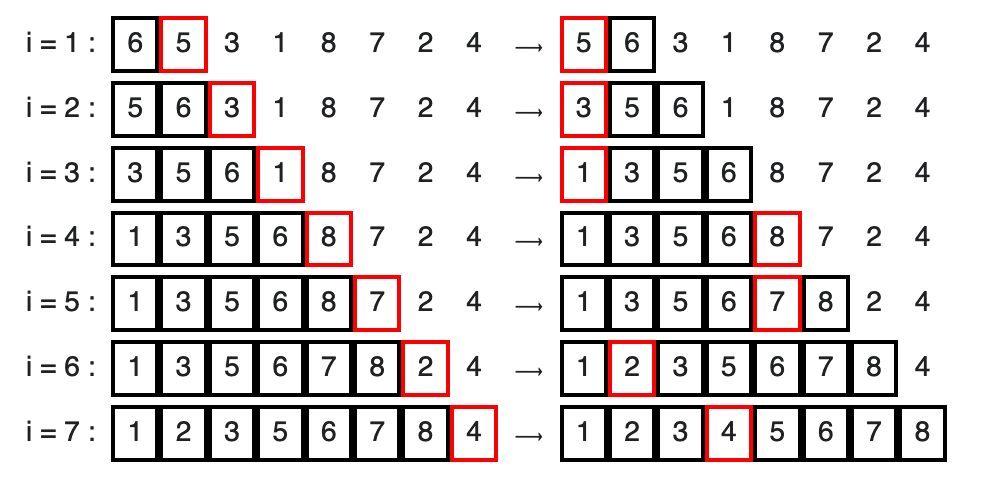
\includegraphics[width=10cm]{ressources/tri_insertion.png}
    \end{figure}

    \begin{solution}
        \textbf{Python :}
            \lstinputlisting{solutions/question10.py} 
        \textbf{Java :}
            \lstinputlisting{solutions/question10.java}
    
    La complexité de l'algorithme est de $O(n^2)$ car nous utilisons 2 boucles imbriquées, qui dans le pire des cas, parcourent la liste deux fois.
    \end{solution}
    
\end{Exercice}


\begin{Exercice} [20 minutes] \textbf{Tri fusion (Merge Sort) - java} \\
    À partir de deux listes triées, on peut facilement construire une liste triée comportant les éléments issus de ces deux listes (leur \textit{fusion}). Le principe de l'algorithme de tri fusion repose sur cette observation : le plus petit élément de la liste à construire est soit le plus petit élément de la première liste, soit le plus petit élément de la deuxième liste. Ainsi, on peut construire la liste élément par élément en retirant tantôt le premier élément de la première liste, tantôt le premier élément de la deuxième liste (en fait, le plus petit des deux, à supposer qu'aucune des deux listes ne soit vide, sinon la réponse est immédiate). 
    
    Les étapes à suivre pour implémenter l'algorithme sont les suivantes:
    \begin{enumerate}
        \item Si le tableau n'a qu'un élément, il est déjà trié.
        \item Sinon, séparer le tableau en deux parties plus ou moins égales.
        \item Trier récursivement les deux parties avec l'algorithme de tri fusion.
        \item Fusionner les deux tableaux triés en un seul tableau trié.
    \end{enumerate}
    
    Soit la liste \lstinline{l} suivante [38, 27, 43, 3, 9, 82, 10], triez les éléments de la liste en utilisant un tri fusion. Combien d'itération effectuez-vous?
    
    \begin{itemize}
        \item \textbf{Java :}
            \lstinputlisting{ressources/question11.java}
    \end{itemize}
    
    \begin{conseil}
    \begin{itemize}
        \item L'algorithme est récursif. 
        \item Revenez à la visualisation de l'algorithme dans les diapositives 83 à 111 pour comprendre comment marche concrètement le tri fusion. 
    \end{itemize}
    
    \end{conseil}
    
     \begin{solution}
        \textbf{Java :}
        \lstinputlisting{striped_files/question11_1.java}
    \end{solution}
    \begin{solution}
        \lstinputlisting{striped_files/question11_2.java}
        
        Le tri fusion est un algorithme récursif. Ainsi, nous pouvons exprimer sa complexité temporelle via une relation de récurrence : $T(n) = 2T(n/2) + O(n)$. En effet, l'algorithme comporte 3 étapes :
        \begin{enumerate}
            \item ``Divide Step'', qui divise les listes en deux sous-listes, et cela prend un temps constant
            \item ``Conquer Step'', qui trie récursivement les sous-listes de taille $n/2$ chacune, et cette étape est représentée par le terme $2T(n/2)$ dans l'équation.
            \item La dernière étape consiste à fusionner les listes, sa complexité est de $O(n)$.
        \end{enumerate}
        La solution à cette équation est $O(n \log n)$.
    \end{solution}
\end{Exercice}

\end{document}



